\documentclass{standalone}
\usepackage{tikz}
\usetikzlibrary{patterns, positioning}


\begin{document}
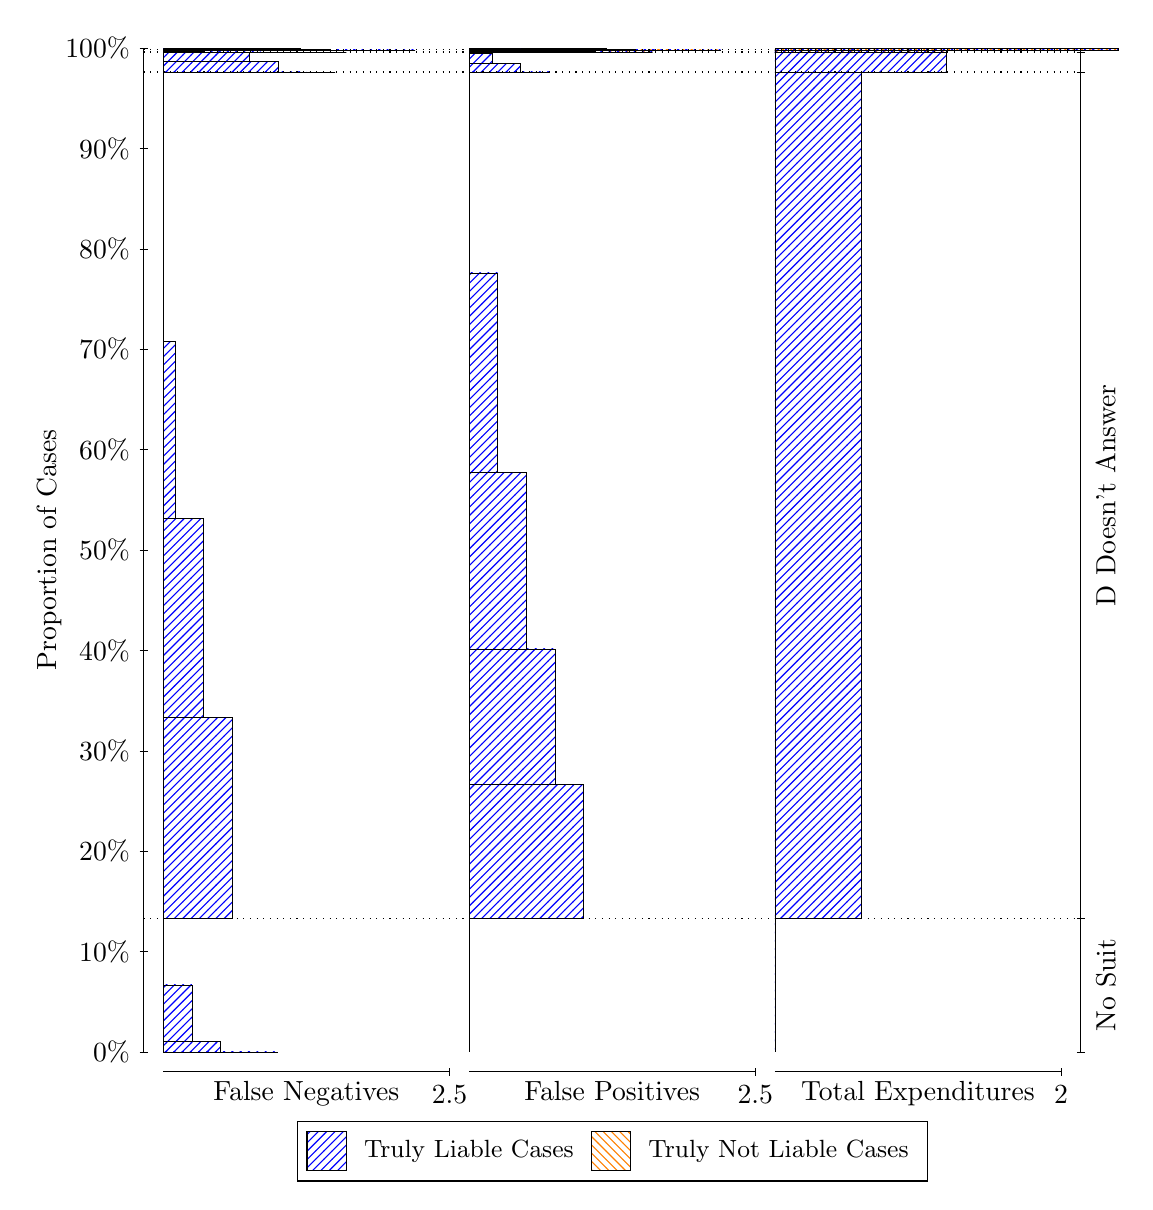
\begin{tikzpicture}
\draw[black, very thin] (1.5,1.75) -- (1.5,14.5);
\node[rotate=90, text=black, anchor=center] at (0.3, 8.125) {Proportion of Cases};
\draw[black, very thin] (1.45,1.75) -- (1.55,1.75);
\node[text=black, anchor=east] at (1.45, 1.75) {0\%};
\draw[black, very thin] (1.45,3.025) -- (1.55,3.025);
\node[text=black, anchor=east] at (1.45, 3.025) {10\%};
\draw[black, very thin] (1.45,4.3) -- (1.55,4.3);
\node[text=black, anchor=east] at (1.45, 4.3) {20\%};
\draw[black, very thin] (1.45,5.575) -- (1.55,5.575);
\node[text=black, anchor=east] at (1.45, 5.575) {30\%};
\draw[black, very thin] (1.45,6.85) -- (1.55,6.85);
\node[text=black, anchor=east] at (1.45, 6.85) {40\%};
\draw[black, very thin] (1.45,8.125) -- (1.55,8.125);
\node[text=black, anchor=east] at (1.45, 8.125) {50\%};
\draw[black, very thin] (1.45,9.4) -- (1.55,9.4);
\node[text=black, anchor=east] at (1.45, 9.4) {60\%};
\draw[black, very thin] (1.45,10.675) -- (1.55,10.675);
\node[text=black, anchor=east] at (1.45, 10.675) {70\%};
\draw[black, very thin] (1.45,11.95) -- (1.55,11.95);
\node[text=black, anchor=east] at (1.45, 11.95) {80\%};
\draw[black, very thin] (1.45,13.225) -- (1.55,13.225);
\node[text=black, anchor=east] at (1.45, 13.225) {90\%};
\draw[black, very thin] (1.45,14.5) -- (1.55,14.5);
\node[text=black, anchor=east] at (1.45, 14.5) {100\%};

\draw[black, very thin] (13.4,1.75) -- (13.4,14.5);
\draw[black, very thin] (13.35,1.75) -- (13.45,1.75);
\node[anchor=west] at (13.35, 1.75) {};
\draw[black, very thin] (13.35,3.4496) -- (13.45,3.4496);
\node[anchor=west] at (13.35, 3.4496) {};
\draw[black, very thin] (13.35,14.195) -- (13.45,14.195);
\node[anchor=west] at (13.35, 14.195) {};
\draw[black, very thin] (13.35,14.441) -- (13.45,14.441);
\node[anchor=west] at (13.35, 14.441) {};
\draw[black, very thin] (13.35,14.451) -- (13.45,14.451);
\node[anchor=west] at (13.35, 14.451) {};
\draw[black, very thin] (13.35,14.477) -- (13.45,14.477);
\node[anchor=west] at (13.35, 14.477) {};
\draw[black, very thin] (13.35,14.5) -- (13.45,14.5);
\node[anchor=west] at (13.35, 14.5) {};

\draw[black, very thin, pattern color=blue, pattern=north east lines] (1.75,1.75) rectangle (3.2033,1.75);
\draw[black, very thin, pattern color=blue, pattern=north east lines] (1.75,1.75) rectangle (2.84,1.7511);
\draw[black, very thin, pattern color=blue, pattern=north east lines] (1.75,1.7511) rectangle (2.4767,1.886);
\draw[black, very thin, pattern color=blue, pattern=north east lines] (1.75,1.886) rectangle (2.1133,2.601);
\draw[black, very thin, pattern color=orange, pattern=north west lines] (1.75,2.601) rectangle (1.75,2.601);
\draw[black, very thin, pattern color=blue, pattern=north east lines] (1.75,2.601) rectangle (1.75,3.4496);
\draw[black, very thin, pattern color=blue, pattern=north east lines] (1.75,3.4496) rectangle (2.622,5.9994);
\draw[black, very thin, pattern color=blue, pattern=north east lines] (1.75,5.9994) rectangle (2.2587,8.5314);
\draw[black, very thin, pattern color=blue, pattern=north east lines] (1.75,8.5314) rectangle (1.8953,10.776);
\draw[black, very thin, pattern color=orange, pattern=north west lines] (1.75,10.776) rectangle (1.75,10.776);
\draw[black, very thin, pattern color=blue, pattern=north east lines] (1.75,10.776) rectangle (1.75,14.195);
\draw[black, very thin, pattern color=blue, pattern=north east lines] (1.75,14.195) rectangle (3.93,14.195);
\draw[black, very thin, pattern color=blue, pattern=north east lines] (1.75,14.195) rectangle (3.5667,14.197);
\draw[black, very thin, pattern color=blue, pattern=north east lines] (1.75,14.197) rectangle (3.2033,14.33);
\draw[black, very thin, pattern color=blue, pattern=north east lines] (1.75,14.33) rectangle (2.84,14.44);
\draw[black, very thin, pattern color=blue, pattern=north east lines] (1.75,14.44) rectangle (2.4767,14.441);
\draw[black, very thin, pattern color=orange, pattern=north west lines] (1.75,14.441) rectangle (1.75,14.441);
\draw[black, very thin, pattern color=blue, pattern=north east lines] (1.75,14.441) rectangle (4.0753,14.441);
\draw[black, very thin, pattern color=blue, pattern=north east lines] (1.75,14.441) rectangle (3.712,14.441);
\draw[black, very thin, pattern color=blue, pattern=north east lines] (1.75,14.441) rectangle (3.3487,14.446);
\draw[black, very thin, pattern color=blue, pattern=north east lines] (1.75,14.446) rectangle (2.9853,14.451);
\draw[black, very thin, pattern color=blue, pattern=north east lines] (1.75,14.451) rectangle (2.622,14.451);
\draw[black, very thin, pattern color=orange, pattern=north west lines] (1.75,14.451) rectangle (1.75,14.451);
\draw[black, very thin, pattern color=blue, pattern=north east lines] (1.75,14.451) rectangle (2.622,14.451);
\draw[black, very thin, pattern color=blue, pattern=north east lines] (1.75,14.451) rectangle (2.2587,14.465);
\draw[black, very thin, pattern color=blue, pattern=north east lines] (1.75,14.465) rectangle (1.8953,14.477);
\draw[black, very thin, pattern color=orange, pattern=north west lines] (1.75,14.477) rectangle (1.75,14.477);
\draw[black, very thin, pattern color=blue, pattern=north east lines] (1.75,14.477) rectangle (1.75,14.477);
\draw[black, very thin, pattern color=blue, pattern=north east lines] (1.75,14.477) rectangle (4.9473,14.477);
\draw[black, very thin, pattern color=blue, pattern=north east lines] (1.75,14.477) rectangle (4.584,14.477);
\draw[black, very thin, pattern color=blue, pattern=north east lines] (1.75,14.477) rectangle (4.2207,14.477);
\draw[black, very thin, pattern color=blue, pattern=north east lines] (1.75,14.477) rectangle (3.8573,14.483);
\draw[black, very thin, pattern color=blue, pattern=north east lines] (1.75,14.483) rectangle (3.494,14.494);
\draw[black, very thin, pattern color=blue, pattern=north east lines] (1.75,14.494) rectangle (3.1307,14.499);
\draw[black, very thin, pattern color=blue, pattern=north east lines] (1.75,14.499) rectangle (2.7673,14.5);
\draw[black, very thin, pattern color=blue, pattern=north east lines] (1.75,14.5) rectangle (2.404,14.5);
\draw[black, very thin, pattern color=blue, pattern=north east lines] (1.75,14.5) rectangle (2.0407,14.5);
\draw[black, very thin, pattern color=orange, pattern=north west lines] (1.75,14.5) rectangle (1.75,14.5);
\draw[black, very thin, pattern color=orange, pattern=north west lines] (5.6333,1.75) rectangle (5.6333,1.75);
\draw[black, very thin, pattern color=blue, pattern=north east lines] (5.6333,1.75) rectangle (5.6333,3.4496);
\draw[black, very thin, pattern color=orange, pattern=north west lines] (5.6333,3.4496) rectangle (7.0867,3.4496);
\draw[black, very thin, pattern color=blue, pattern=north east lines] (5.6333,3.4496) rectangle (7.0867,5.1496);
\draw[black, very thin, pattern color=blue, pattern=north east lines] (5.6333,5.1496) rectangle (6.7233,6.8686);
\draw[black, very thin, pattern color=blue, pattern=north east lines] (5.6333,6.8686) rectangle (6.36,9.1129);
\draw[black, very thin, pattern color=blue, pattern=north east lines] (5.6333,9.1129) rectangle (5.9967,11.645);
\draw[black, very thin, pattern color=blue, pattern=north east lines] (5.6333,11.645) rectangle (5.6333,14.195);
\draw[black, very thin, pattern color=orange, pattern=north west lines] (5.6333,14.195) rectangle (6.6507,14.195);
\draw[black, very thin, pattern color=blue, pattern=north east lines] (5.6333,14.195) rectangle (6.6507,14.196);
\draw[black, very thin, pattern color=blue, pattern=north east lines] (5.6333,14.196) rectangle (6.2873,14.306);
\draw[black, very thin, pattern color=blue, pattern=north east lines] (5.6333,14.306) rectangle (5.924,14.438);
\draw[black, very thin, pattern color=blue, pattern=north east lines] (5.6333,14.438) rectangle (5.6333,14.441);
\draw[black, very thin, pattern color=orange, pattern=north west lines] (5.6333,14.441) rectangle (6.5053,14.441);
\draw[black, very thin, pattern color=blue, pattern=north east lines] (5.6333,14.441) rectangle (6.5053,14.441);
\draw[black, very thin, pattern color=blue, pattern=north east lines] (5.6333,14.441) rectangle (6.142,14.446);
\draw[black, very thin, pattern color=blue, pattern=north east lines] (5.6333,14.446) rectangle (5.7787,14.451);
\draw[black, very thin, pattern color=blue, pattern=north east lines] (5.6333,14.451) rectangle (5.6333,14.451);
\draw[black, very thin, pattern color=orange, pattern=north west lines] (5.6333,14.451) rectangle (7.9587,14.451);
\draw[black, very thin, pattern color=blue, pattern=north east lines] (5.6333,14.451) rectangle (7.9587,14.451);
\draw[black, very thin, pattern color=blue, pattern=north east lines] (5.6333,14.451) rectangle (7.5953,14.451);
\draw[black, very thin, pattern color=blue, pattern=north east lines] (5.6333,14.451) rectangle (7.232,14.463);
\draw[black, very thin, pattern color=blue, pattern=north east lines] (5.6333,14.463) rectangle (6.8687,14.477);
\draw[black, very thin, pattern color=blue, pattern=north east lines] (5.6333,14.477) rectangle (6.5053,14.477);
\draw[black, very thin, pattern color=orange, pattern=north west lines] (5.6333,14.477) rectangle (8.8307,14.477);
\draw[black, very thin, pattern color=blue, pattern=north east lines] (5.6333,14.477) rectangle (8.8307,14.477);
\draw[black, very thin, pattern color=blue, pattern=north east lines] (5.6333,14.477) rectangle (8.4673,14.477);
\draw[black, very thin, pattern color=orange, pattern=north west lines] (5.6333,14.477) rectangle (8.4673,14.477);
\draw[black, very thin, pattern color=blue, pattern=north east lines] (5.6333,14.477) rectangle (8.4673,14.477);
\draw[black, very thin, pattern color=blue, pattern=north east lines] (5.6333,14.477) rectangle (8.104,14.477);
\draw[black, very thin, pattern color=orange, pattern=north west lines] (5.6333,14.477) rectangle (8.104,14.477);
\draw[black, very thin, pattern color=blue, pattern=north east lines] (5.6333,14.477) rectangle (8.104,14.477);
\draw[black, very thin, pattern color=blue, pattern=north east lines] (5.6333,14.477) rectangle (7.7407,14.477);
\draw[black, very thin, pattern color=orange, pattern=north west lines] (5.6333,14.477) rectangle (7.7407,14.477);
\draw[black, very thin, pattern color=blue, pattern=north east lines] (5.6333,14.477) rectangle (7.7407,14.483);
\draw[black, very thin, pattern color=blue, pattern=north east lines] (5.6333,14.483) rectangle (7.3773,14.483);
\draw[black, very thin, pattern color=orange, pattern=north west lines] (5.6333,14.483) rectangle (7.3773,14.483);
\draw[black, very thin, pattern color=blue, pattern=north east lines] (5.6333,14.483) rectangle (7.3773,14.494);
\draw[black, very thin, pattern color=blue, pattern=north east lines] (5.6333,14.494) rectangle (7.014,14.499);
\draw[black, very thin, pattern color=blue, pattern=north east lines] (5.6333,14.499) rectangle (6.6507,14.5);
\draw[black, very thin, pattern color=blue, pattern=north east lines] (5.6333,14.5) rectangle (6.2873,14.5);
\draw[black, very thin, pattern color=blue, pattern=north east lines] (5.6333,14.5) rectangle (5.924,14.5);
\draw[black, very thin, pattern color=orange, pattern=north west lines] (9.5167,1.75) rectangle (9.5167,1.75);
\draw[black, very thin, pattern color=blue, pattern=north east lines] (9.5167,1.75) rectangle (9.5167,3.4496);
\draw[black, very thin, pattern color=orange, pattern=north west lines] (9.5167,3.4496) rectangle (10.607,3.4496);
\draw[black, very thin, pattern color=blue, pattern=north east lines] (9.5167,3.4496) rectangle (10.607,14.195);
\draw[black, very thin, pattern color=orange, pattern=north west lines] (9.5167,14.195) rectangle (11.697,14.195);
\draw[black, very thin, pattern color=blue, pattern=north east lines] (9.5167,14.195) rectangle (11.697,14.441);
\draw[black, very thin, pattern color=orange, pattern=north west lines] (9.5167,14.441) rectangle (11.697,14.441);
\draw[black, very thin, pattern color=blue, pattern=north east lines] (9.5167,14.441) rectangle (11.697,14.451);
\draw[black, very thin, pattern color=orange, pattern=north west lines] (9.5167,14.451) rectangle (11.697,14.451);
\draw[black, very thin, pattern color=blue, pattern=north east lines] (9.5167,14.451) rectangle (11.697,14.477);
\draw[black, very thin, pattern color=orange, pattern=north west lines] (9.5167,14.477) rectangle (13.877,14.477);
\draw[black, very thin, pattern color=blue, pattern=north east lines] (9.5167,14.477) rectangle (13.877,14.477);
\draw[black, very thin, pattern color=orange, pattern=north west lines] (9.5167,14.477) rectangle (13.877,14.477);
\draw[black, very thin, pattern color=blue, pattern=north east lines] (9.5167,14.477) rectangle (13.877,14.5);
\draw[black, dotted] (1.5,3.4496) -- (13.4,3.4496);
\draw[black, dotted] (1.5,14.195) -- (13.4,14.195);
\draw[black, dotted] (1.5,14.441) -- (13.4,14.441);
\draw[black, dotted] (1.5,14.451) -- (13.4,14.451);
\draw[black, dotted] (1.5,14.477) -- (13.4,14.477);
\draw[black, very thin] (1.75,1.5) -- (5.3833,1.5);
\node[text=black, anchor=north] at (3.5667, 1.5) {False Negatives};
\draw[black, very thin] (5.3833,1.45) -- (5.3833,1.55);
\node[text=black, anchor=north] at (5.3833, 1.45) {2.5};

\draw[black, very thin] (5.6333,1.5) -- (9.2667,1.5);
\node[text=black, anchor=north] at (7.45, 1.5) {False Positives};
\draw[black, very thin] (9.2667,1.45) -- (9.2667,1.55);
\node[text=black, anchor=north] at (9.2667, 1.45) {2.5};

\draw[black, very thin] (9.5167,1.5) -- (13.15,1.5);
\node[text=black, anchor=north] at (11.333, 1.5) {Total Expenditures};
\draw[black, very thin] (13.15,1.45) -- (13.15,1.55);
\node[text=black, anchor=north] at (13.15, 1.45) {2};

\node[text=black, centered, rotate=90] at (13.72, 2.5998) {No Suit};
\node[text=black, centered, rotate=90] at (13.72, 8.8221) {D Doesn't Answer};





\draw (7.449999999999999,1.5) node[draw=none] (baseCoordinate) {};
\begin{scope}[align=center]
        \matrix[scale=0.5, draw=black, below=0.5cm of baseCoordinate, nodes={draw}, column sep=0.1cm]{
            \node[rectangle, draw, minimum width=0.5cm, minimum height=0.5cm, pattern color=blue, pattern=north east lines] {}; &
            \node[draw=none, font=\small, text=black] (B) {Truly Liable Cases}; &
            \node[rectangle, draw, minimum width=0.5cm, minimum height=0.5cm, pattern color=orange, pattern=north west lines] {}; &
            \node[draw=none, font=\small, text=black] (B) {Truly Not Liable Cases}; \\
            };
\end{scope}

\end{tikzpicture}
\end{document}